\documentclass[]{article}
\usepackage{graphicx}
\usepackage{float}
\usepackage{amsmath,amssymb,amsthm} % For including math equations, theorems, symbols, etc
\usepackage{subfig}
\graphicspath{{Figures/}} 
\usepackage{hyperref}
\PassOptionsToPackage{dvipsnames}{xcolor}
\RequirePackage{xcolor} % [dvipsnames]
\definecolor{CTsemi}{gray}{0.55} % chapter numbers will be semi transparent .5 .55 .6 .0
\definecolor{CTcitation}{rgb}{0,0.5,0} % WebGreen
\definecolor{CTurl}{named}{Maroon} % Maroon
\definecolor{CTtitle}{named}{Maroon} % Maroon {cmyk}{0, 0.87, 0.68, 0.32}
\definecolor{CTlink}{named}{RoyalBlue} % RoyalBlue {cmyk}{1, 0.50, 0, 0}
\definecolor{halfgray}{gray}{0.55} % chapter numbers will be semi transparent .5 .55 .6 .0
\definecolor{webgreen}{rgb}{0,0.5,0}
\definecolor{webbrown}{rgb}{0.6,0,0}
\hypersetup{
	colorlinks=true,
	linkcolor=RoyalBlue,
	filecolor=magenta,      
	urlcolor=cyan,
	pdfkeywords={}
	breaklinks=true, bookmarks=true,bookmarksnumbered,
	urlcolor=webbrown, citecolor=webgreen, % Link colors
	pdftitle={}, % PDF title
	pdfauthor={\textcopyright}, % PDF Author
	pdfsubject={}, % PDF Subject
	pdfkeywords={}, % PDF Keywords
	pdfcreator={pdfLaTeX}, % PDF Creator
	pdfproducer={LaTeX with hyperref and ClassicThesis} % PDF producer
}

%opening
\title{Bayesian Evidence Synthesis:opioid crisis}
\author{Hyeongcheol Park* \& Paul Gustafson* \& Micheal A Irvine*\textsuperscript{1}}

\begin{document}
%\renewcommand{\sectionmark}[1]{\markright{\spacedlowsmallcaps{#1}}}
\maketitle{}
\tableofcontents % Print the table of contents
\listoffigures % Print the list of figures
\listoftables % Print the list of tables


\begin{abstract}

\end{abstract}

\section{Introduction}
The opioid crisis is a major issue in North America including British Columbia, Canada. British Columbia is in the midst of a drug overdose crisis due to illicit opioids and the circumstance is getting worse; According to the BC Coroners Service, there were more than 930 apparent illicit drug overdose deaths in BC from Jan. 1 to Dec. 31, 2016. This compares to 518 in 2015, an increase of 79.2\%. \cite{bccdc_opioid}  The goal of this project is to apply Bayesian evidence synthesis to understand better the opoid crisis in British Columbia, Canada.  \\ 

One difficulty to cope with the opioid crisis is that the total number of overdoses is unknown. The reason is that the use of prescription opioids often leads to use illicit opioids and the illicit usage cannot be known. Many of those who become addicted to opioids do so after initially receiving a prescription. The highly addictive nature of these pain relievers makes it easy for the human brain to crave more. It is only after their prescription ends that many users realize they’ve become dependent on the effects of opioids  to function “normally.” At that point, they are either forced to get clean and endure the pain that comes with the withdrawal symptoms of opioids or look for another means of getting their high. This is often the time where people will turn to illicit drugs or other analogues. Because prescription opioids are so expensive, this is when many users turn to heroin. It is often cheaper, more potent, and easier to locate than what they were taking before. In fact, about 80\% of people using heroin started with a prescription to another opioid. After using heroin, however, 23\% of individuals develop opioid addiction.\cite{opioid_desc} [attempt: need to give a backstory-why isn't this observable? The number of overdoses]\\

Since the total overdoses are unknown, the number needs to be estimated. Bayesian statistics can be a way to approach the problem and give us the good estimate of the number. Bayesian statistics is a theory in the field of statistics based on the Bayesian interpretation of probability where probability expresses a degree of belief in an event. \cite{wiki_bayes} Detailed explanation is provided at the following section. [attempt: explain Bayesian statistics]\\

All examples here were performed in Python 3.7 using the library pyMC (reference) and JAGS (reference). Training was performed using No U-Turn Sampling (NUTS) over two chains with 1000 iterations (is it sample size?). Fitting was performed on a GHz Intel Core i5 with 8GM of LPDD3 RAM and typically had wall times under ten minutes. Data processing was carried out using the Pandas and SciPy library [reference]. Data visualization was performed using the libraries Seaborn and Matplotlib [ref]. Code for all examples in this study are provided. \\

\section{methods}

\normalsize

The number of overdoses is our ultimate interest of estimation. To achive the goal in context of Bayesian statistics, we use our prior belief and available data set about the target of estimation. The posterior belief is coming from both parts of the information. Following equation express the idea in a mathmatical form:  
\begin{equation}
\label{bayes_thm}
\left.\begin{aligned}
p(\theta| y ) = \frac{ p(\theta, y)   }{ p(y)} = \frac{ p(\theta) p(y| \theta)}{ p(y)} \propto p(\theta) p(y| \theta) \end{aligned}\right.
\end{equation}
where $\theta$ represents the target of estimation, the total overdoses and $y$ represents the collected data set providing relevant samples of the target variable. In Bayesian concepts, the variable of interest $\theta$ is a fixed number but the number is yielded from a certain distribution; That is, $\theta$ is considered to be a sample of a random variable. The problem, however, is that the data $y$ is not available. We can have our prior belief about the total overdoses but it is not possible to obtain any data. Hence it is needed to approach the estimation in a indirect fashion. Figure \ref{simple_draw} shows an example of how the estimation can be proceeded. [attempt: Give a graphical model representation? state that(?)]
\begin{figure}[htb]
	\centering
	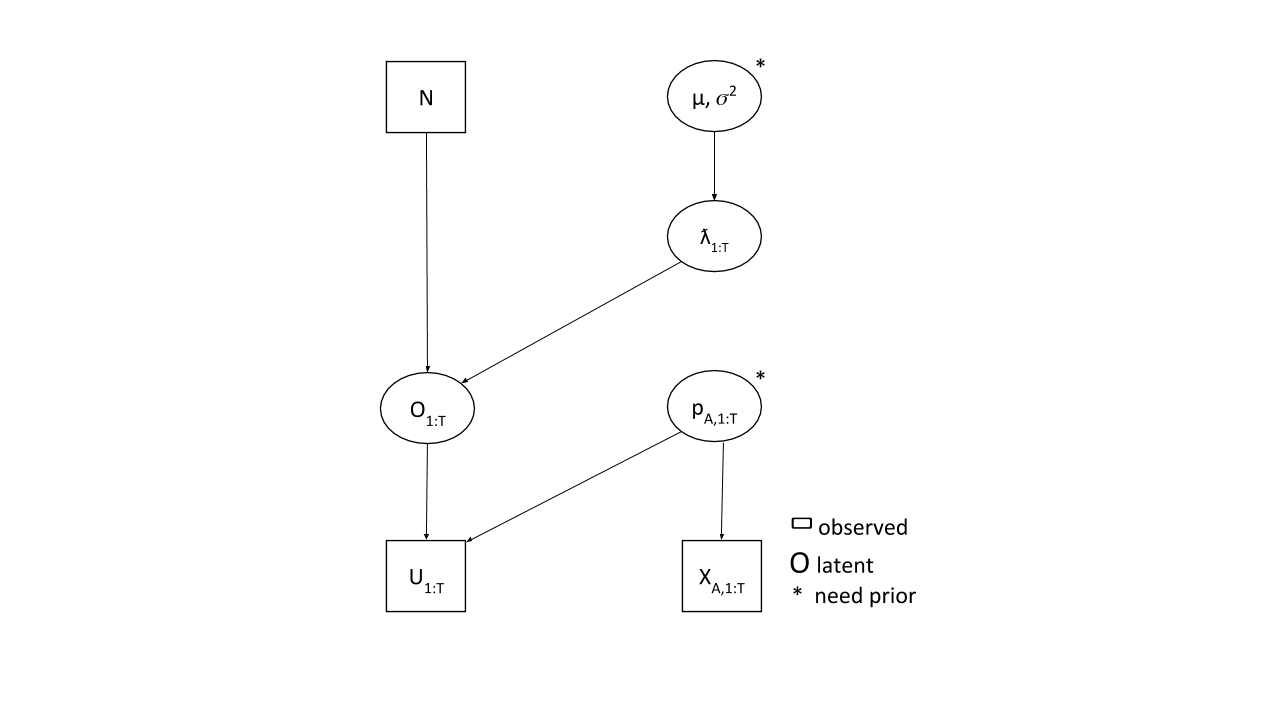
\includegraphics[width=0.5\linewidth]{Figures/simple_drawing}
	\caption{Example of estimating the total overdoses indirectly given two data sets: ambulance attended overdoses and survey data. N is the population size}
	\label{simple_draw}
\end{figure}
\\

 Let $O_t$ the number of overdoses in a given month $t$ in British Columbia. [attempt: specify a geographic area] Suppose there was a survey  conducted to estimate the proportion of ambulance call $p_A$ among the overdoses. $p_A$ is assumed constant across time for simplicity. Let $n_{A}$ the sample size of the survey and $x_{A}$ to be the total number who confirmed they did call ambulance. It is assumed that $x_{A}$ follows a Binomial distribution:

\begin{equation}
\label{ambulance}
\left.\begin{aligned}
x_{A} \sim Bin(n_{A},p_{A})\end{aligned}\right.
\text{ambulance call-outs model}
\end{equation}

The total overdoses need to be modeled. The simplest conceptual model is to take an underlying log-rate $z_t$ that is independent and identically distributed across months according to a normal distribution with mean $\mu$ and variance $\sigma^2$. \cite{Irvine:modelling} Denote $\lambda_{t}^{OD}$ the rate of overdose at time $t$. It is assumed that the total overdose $O_t$ follows Poisson distribution where the population of the region of interest is $N$. 

\begin{equation}
\label{overdose}
\left.\begin{aligned}
z_{t} \sim N(\mu, \sigma^{2}) \\
\lambda_{t}^{OD} = \exp(z_{t})\\
O_{t} \sim Poi(\lambda_{t}^{OD}N) 
\end{aligned}\right\} 
\text{		overdose model} 
\end{equation}

Estimation of $O_t$ is not straightforward since none of the variables ($\mu$, $\sigma$, $N$) determining $O_t$  is known. Hence $O_t$ should be inferred from using $U_t$ and \(p_A\), where $p_A$ is the ambulance call out rate and \(U_t\) is the number of  ambulance-attended overdoses at a time point $t$. In general, the data of ambulance-attended overdoses \(U_t\) can be obtained. It is assumed that  \(U_t\) follows Binomial distribution: 
\begin{equation}
\label{over_amb}
\left.
U_t \sim Bin(O_t, p_A)
\right.
\end{equation}

Now $O_t$ can be estimated as $p_A$ can be infered by survey data and the data regarding $U_t$ is given. We suggest a simple model as a start where the model only combines Ambulance Call-outs Model (\ref{ambulance}) and Overdose Model (\ref{overdose}). 

The next step is to run some simulations to figure out how different types of inputs lead some changes of output. To do so, the simple model is illustrated below.\\

\subsection{Simulation}

\normalsize 
The first simulation simplifies the assumptions of variables as much as possible; we assumed $N= 10000, n_{A}=1000$. Note that the population size, N,  is unknown in reality but it is assumed known for the investigator here for simplicity as in figure \ref{simple_draw}. The assumptions will change later to see the impact of the likelihood over the posterior distributions of variables of interest; the total population size for a region, N, could vary over time or it can be staritified for a better realization of the reality. The survey size could also vary such as $n_{A}=100$ or $n_{A}=10000$ in later examples.  \\

\subsubsection{Markov chain Monte Carlo}
The achievement of the simulation was done by Markov chain Monte Carlo (MCMC). The technique is a popular method to obtain posterior samples from distributions where analytic forms do not exist or are hard to be derived. \textbf{[Further explanation is going to be added.]} [attempt:brief explaination of MCMC and related topics]\\


\subsubsection{Likelihood}

\normalsize 
There exist two data sets; survey data ($n_A, x_A$), and ambulance attended overdose data ($U_t$). The two data sets are simulated as follows. 
The true value of $p_A$ was set $p_A=0.8$ for the survey data.
It is assumed that the data was collected for a year (t=1,2,3, ..., 12) and 
$x_t$ values were independentally generated from the Binomial distribution (\ref{ambulance}).  In terms of overdose data, It is assumed that the true values of parameters for overdose model were $\mu=\log0.05,\ \sigma=1$.
The vector of $O_t$ was generated following the overdose model (\ref{overdose}). The vector of $U_t$ was generated from the Binomial relation of the two variables ($\ref{over_amb}$). The two generated vectors have the same length with the survey data (t=1,2,3, ..., 12). [Delete: Then the 12 sueveys were combined into a single survey since $p_A$ is assumed fixed across time in this contexts.] Note that only $U_t$ and $x_t$ are known as the likelihood and $p_A$ needs to be estimated first so as to estimate $O_t$ which is the ultimate interest of the research.\\


\subsubsection{Prior Distributions}
\normalsize Noninformative prior distributions are presumed as a start for simplicity. 

\begin{equation}
\label{nonin_prior_amb}
p(p_A) \sim Beta(1,1)
\text{			noninformative prior of ambulance model}
\end{equation} 

\begin{equation}
\label{noninprior_over}
\left.\begin{aligned}
\mu \sim U(-10,0)\\
\sigma \sim U(0,5)
\end{aligned}\right\} 
\text{			noninformative prior of overdose model}
\end{equation}

This leads the posterior distribution of variables of interest to heavily depend on the likelihood. Later, the noninformative priors will be changed and the impact of the changes over posteriors will be investigated. \\

\subsection{Early Result } 

The result from the simple case scenario is illustrated below.

\subsubsection{Posterior Distribution}


Figure \ref{pst_ot} is the boxplot of posterior samples of $O_t$. It is shown that our posterior estimates of  $O_t$ are fairly accurate since (1) the boxplots contain actual values of $O_t$ within their interquartile range (IQR) and (2) the ranges of IQR and 95\% range seem narrow. Notice that the range of the boxplot from a higher $O_t$ values (t=1, 7, 11) is wider than the other ranges of the boxplots from smaller estimates of $O_t$ (all t values but 1, 7, 11)\\

\begin{figure}[h]
	\centering
	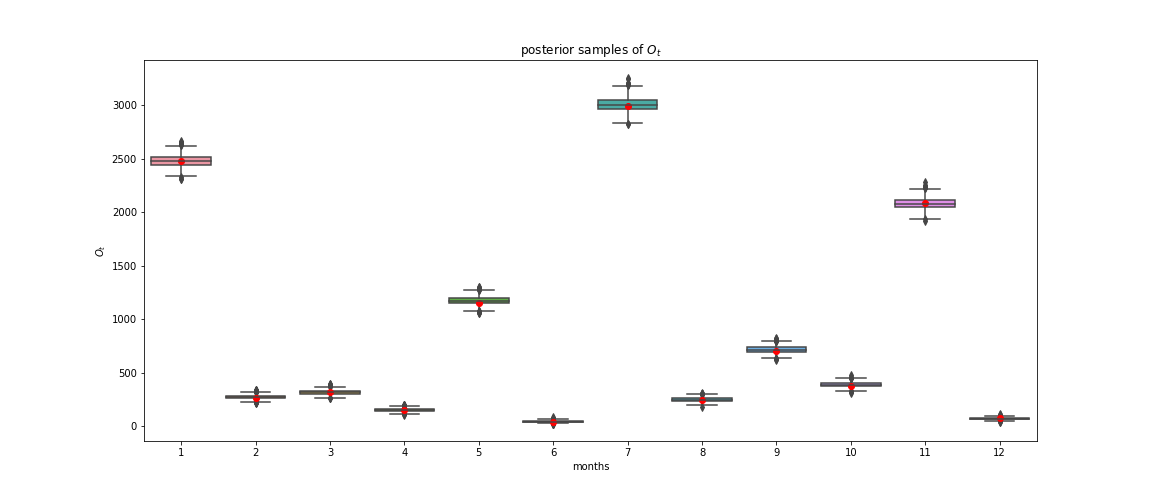
\includegraphics[width=1\linewidth]{Figures/earlyresult1_ot.png}
	\caption{Boxplot of posterior samples of $O_t$ (2000 samples for each month) with actual data points of simulated $O_t$ values. The simulated values are shown as red dots.}
	\label{pst_ot}
\end{figure}

\newpage
\subsubsection{Posterior Predictive Check}
Posterior predictive checking is a model validation technique that we simulate some replicated data under the fitted model then compare the new data to the observed data. If the model fits, then replicated data generated under the model should look similar to observed data. To put it another way, the observed data should look plausible under the posterior predictive distribution. This is really a self-consistency check: an observed discrepancy can be due to model misfit or chance. \cite{bda_galman}
[attempted: brief explannation of what is PPC]\\

Figure \ref{ppc_ut} is the boxplot of posterior predictive samples of $U_t$. It is shown that the posterior predictive estimates of $U_t$ is failry accurate with the same two reasons regarding the accuracy of the posterior distribution of $O_t$. It is more obvious here that the range of the boxplots from higher $O_t$ values (t=1, 7, 11) is wider than the other ranges of the boxplots from smaller estimates of $O_t$ (all t values but 1,7, 11). Notice that the relative ranges of figure \ref{ppc_ut} follow the ones of figure \ref{pst_ot}; for months where $U_t$ values are higher, the values of $O_t$ are also higher than the average (t=1, 7, 11)\\

\begin{figure}[htb]
	\centering
	\subfloat[ppc of $U_t$]{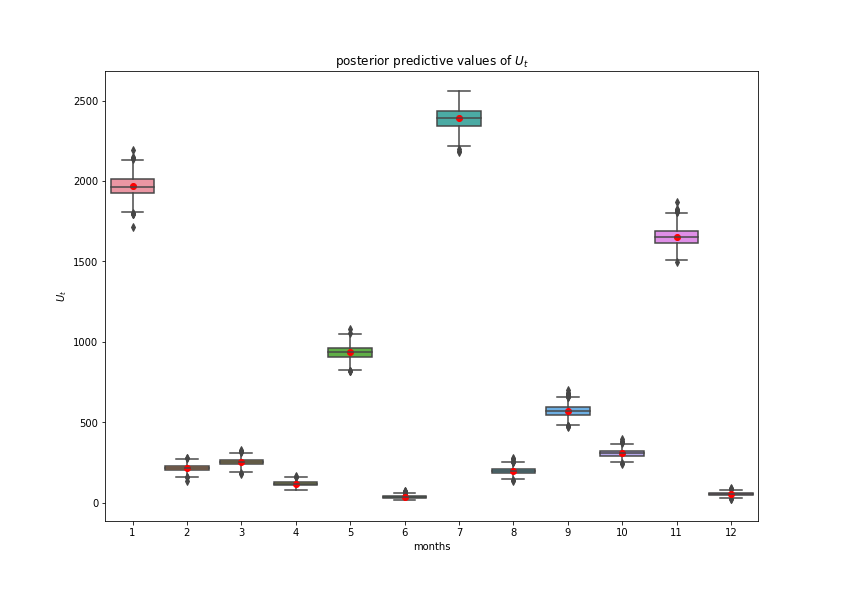
\includegraphics[width=.50\columnwidth]{Figures/early_r_ppc1_ut.png}\label{ppc_ut}}
	\subfloat[ppc of $p_A$]{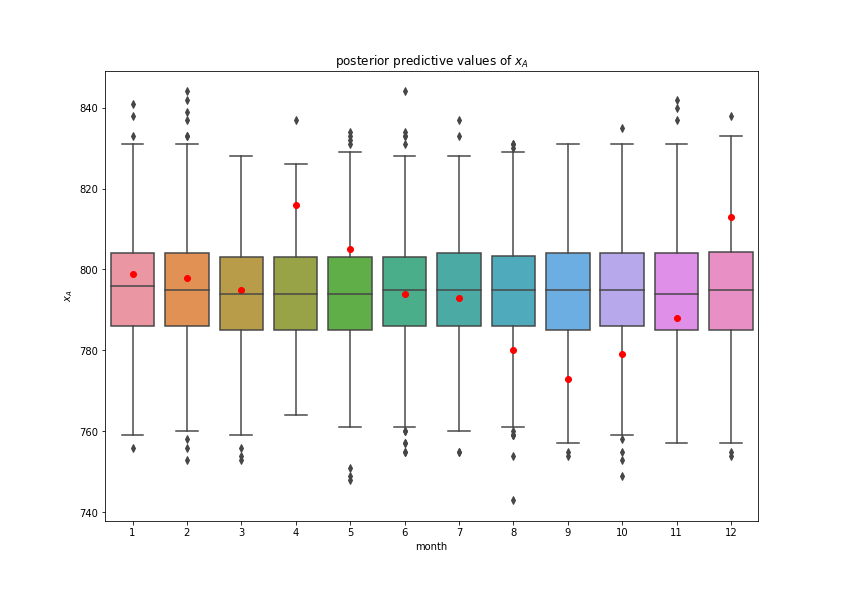
\includegraphics[width=.50\columnwidth]{early_r_ppc1_xt}\label{ppc_xt}}
	\caption[two early result box plots:]{Boxplots of posterior predictive samples of $x_A$ (1000 samples) with the actual data point of simulated $U_t$,$x_A$ value. The simulated values are shown as a red dots.}
	
\end{figure}

Figure \ref{ppc_xt} is the boxplots of posterior predictive samples of $x_A$. It is shown that the posterior predictive estimates of $x_A$ is tolerably accurate since (1) the boxplots contain actual values of $O_t$ within their lines connecting the maximum and the minimum and (2) the ranges of IQR seem modereately narrow. \\



\subsection{Early Result: Contamination of $p_A$ } 
One of the attention of this research project is to investigate how robust the model is from contaminations of the data sets. The first inspection is to check an impact of a contamination of $p_A$; what would happen if the estimation of $p_A$ is biased? It is assumed that the survey data gives us a wrong estimate of $p_A$ such that it would be underestimated or overestimated. We then want to see how the biased estimation of $p_A$ affects the estimate of $O_t$, the total overdose.\\

Both of underestimation and overestimation were conducted for the analysis. In terms of underestimation, the simulated survey data ($n_A, x_A$) was generated with $p_A=0.6$ while the true value of $p_A$ is 0.8, and all the other assumptions hold the same. That is, $x_A$ is generated from $x_A \sim Bin(n_A, 0.6)$, while $U_t$ is generated from $U_t \sim Bin(O_t, 0.8)$ for every $t$. For overestimation, the simulated survey data was generated with $p_A=0.9$ while the true value of $p_A$ is 0.8, and all the other assumptions hold the same.  \\

\subsubsection{Posterior Distribution}

\begin{figure}[htb]
	\centering
	\subfloat[ppc of $O_t$: underestimated $p_A$]{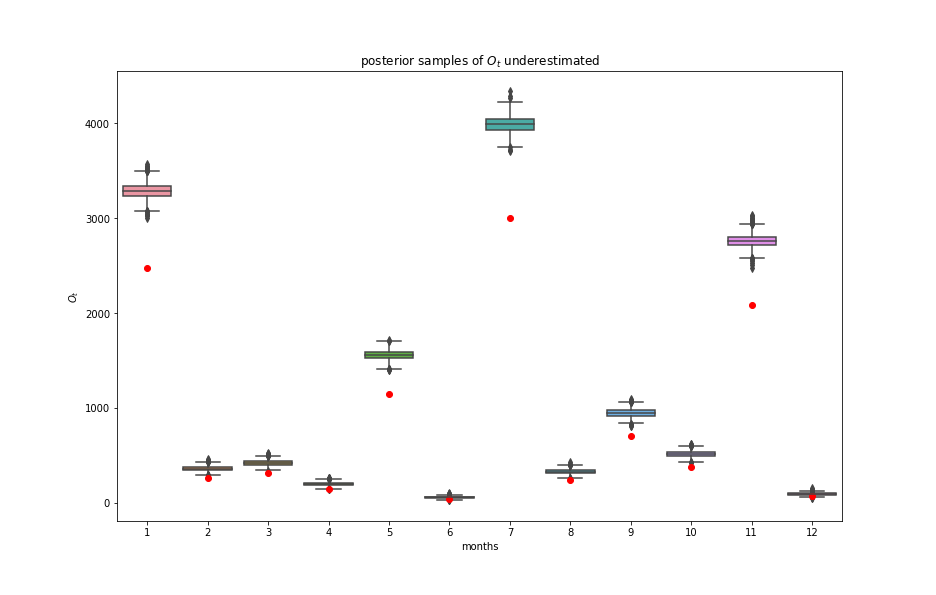
\includegraphics[width=.50\columnwidth]{early_contamination_underestimated-o_t.png}\label{under_ot}}
	\subfloat[ppc of $O_t$: overestimated $p_A$]{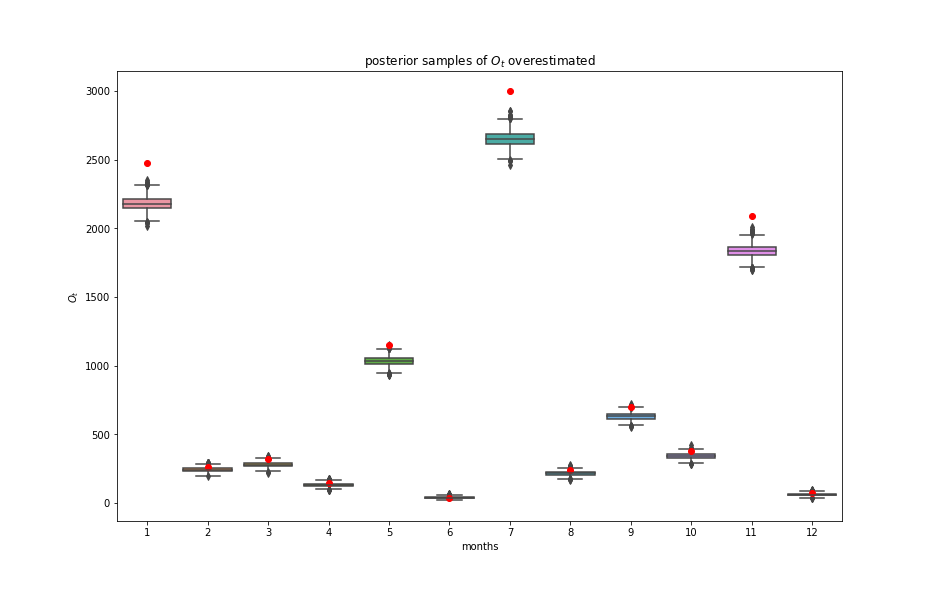
\includegraphics[width=.50\columnwidth]{early_contamination_overestimated-o_t}\label{over_ot}}
	\caption[two early result box plots:]{Boxplot of posterior samples of $O_t$ (1000 samples) where survey data is contaminated.  The actual data point of simulated $O_t$ values are shown as red dots.}
	\label{contam_ot}
\end{figure}

\normalsize 
Figure \ref{contam_ot} is the boxplots of posterior samples where $p_A$ is contaminated from the survey data. It is seen that the underestimation of $p_A$ (\ref{under_ot}) leads to an overestimation of $O_t$ as the boxplots are above the red dots. This is justifiable considering the given data sets (likelihoods) and the relationship between the two models (\ref{over_amb}); given the likelihood of the ambulance attended overdoses, $U_t$, a value of $O_t$ is an unknown parameter of the binomial distribution, $Bin(O_t, p_A)$. Let $o_t$, $u_t$ are samples from $O_t$ and the likelihood value of $U_t$ respectively. Then $o_t$ is proportional to the quantity generated by multiplying $u_t$ and the inverse of $\hat{p}_{A}$ where $\hat{p}_{A}$ is underestimated estimator of $p_A$; hence $\frac{1}{\hat{p}_{A}}$ is overestimated which leads overestimation of $O_t$.
\begin{equation}
\label{ot.how.made}
\begin{aligned}
o_t \propto u_t \frac{1}{\hat{p}_{A}}
\end{aligned}
\end{equation}
Figure \ref{over_ot} shows the opposite case. Overestimation of $p_A$ leads underestimation of the inverse of $p_A$ which causes underestimation of $O_t$. From both figures it is seen that the bias increases as the estimated values and the actual values get large.\\

\subsubsection{Posterior Predictive Check}

Figure \ref{contam_ut} are the boxplots of posterior predictive samples where $p_A$ is underestimated and overestimated respectively from the survey data. It is seen that none of the contaminations of $p_A$ leads an contamination effect on $U_t$ but only affects the $O_t$ estimation.\\

The possible explanation is that the contaminations of  $p_A$ and $O_t$ (from $p_A$) cancel out the bias component as combined so that $U_t$ has no bias. Notice that $U_t$ is a likelihood (data set) of $O_t$ estimation. Hence it plays the role of $y$ in Bayes theorem (\ref{bayes_thm}) and the likelihood, $U_t$, is used to obtain the biased posterior samples of $O_t$ with the contaminated estimates of $p_A$. Here the pair of $(O_t, P_A)$ are both biased and the pair is fitted by the likelihood, $U_t$. To obtain the posterior predictive samples, MCMC algorithm help obtain posterior samples of biased $O_t$ and then the samples will be combined with biased $p_A$ such that the new samples of $\tilde{U_t}$ from $p(\tilde{U_t}|{U_t})$ is obtained.  The result also matches with our intution. Posterior predictive checkes use the existing data points twice; firstly it uses the data to obtain the posterior samples of paramaters, and secondly the samples are used to produce posterior predictive samples. Given the fact that there could be an overfitting issue due to using the data twice, the result shown here seems reasonable. 
\\

\begin{figure}[htb]
	\centering
	\subfloat[ppc of $U_t$: underestimated $p_A$]{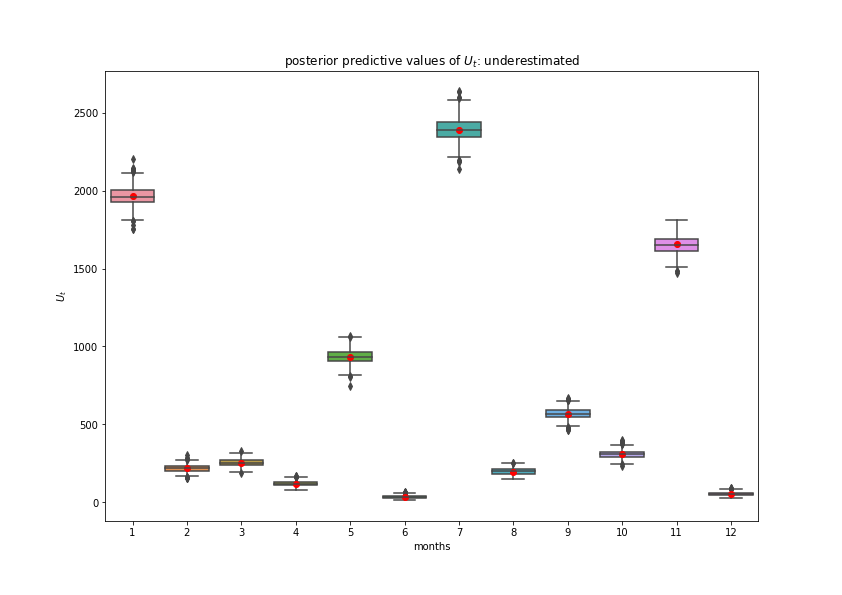
\includegraphics[width=.50\columnwidth]{early_contamination_underestimated-u_t.png}\label{under_ut}}
	\subfloat[ppc of $U_t$: overestimated $p_A$]{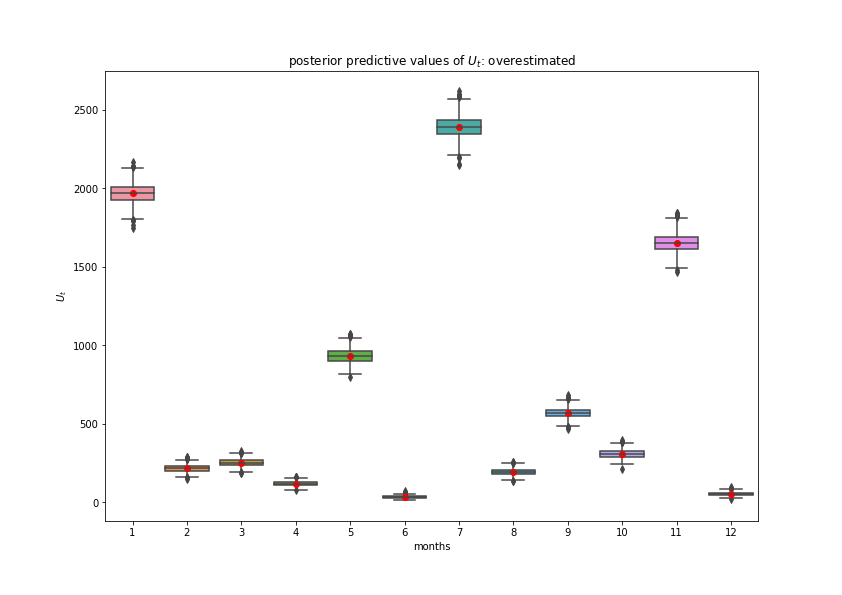
\includegraphics[width=.50\columnwidth]{early_contamination_overestimated-u_t}\label{over_ut}}
	\caption[two early result box plots:ut]{Boxplot of posterior samples of $U_t$ (1000 samples) where survey data is contaminated.  The actual data point of simulated $U_t$ values are shown as red dots.}
	\label{contam_ut}
\end{figure}

Figure \ref{contam_xt}  are the boxplots of posterior predictive samples of $x_A$ where $p_A$ is underestimated and overestimated respectively from the survey data. It is seen that none of the contaminations of $p_A$ leads an effect of contamination on $x_A$; the actual simulated points (red dots) are close to the medians from the two boxplots. However, notice that the range of the estimated values are different between the two boxplots; the median from Figure \ref{under_xa} is around 600 whereas the median from Figure \ref{over_xa} is around 900. [???? I think this should go to the previous of the previous paragraph] This is because overdose model (\ref{overdose}) does not affect the resulf from the ambulance model (\ref{ambulance}); only the ambulance model has an effect on the overdose model.

\begin{figure}[h]
	\centering
	\subfloat[ppc of $x_A$: underestimated $p_A$]{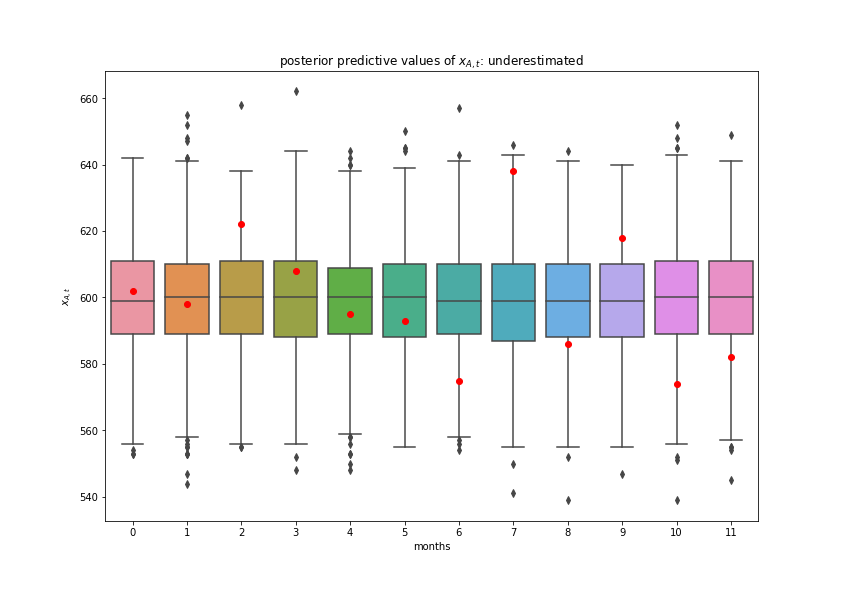
\includegraphics[width=.50\columnwidth]{early_contamination_underestimated-x_a.png}\label{under_xa}}
	\subfloat[ppc of $x_A$: overestimated $p_A$]{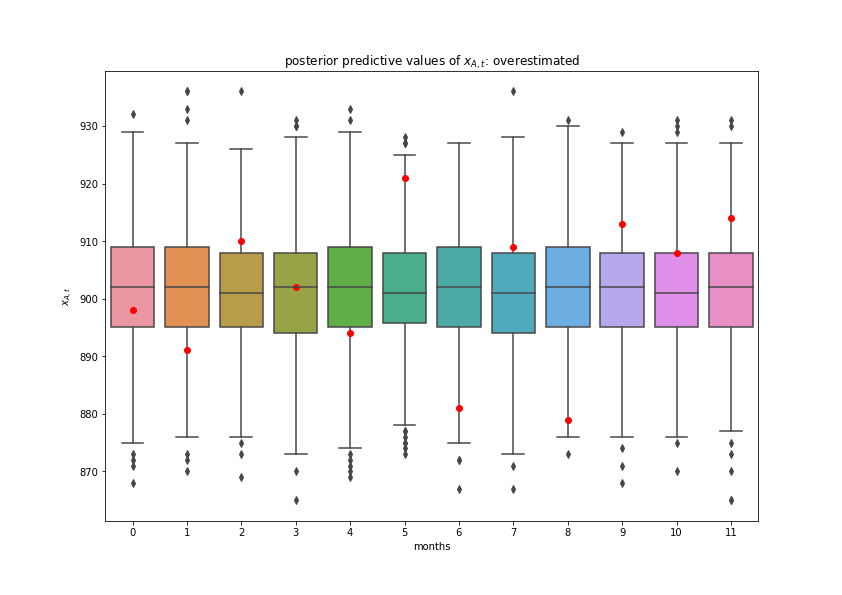
\includegraphics[width=.50\columnwidth]{early_contamination_overestimated-x_a.png}\label{over_xa}}
	\caption[two early result box plots:xa]{Boxplot of posterior samples of $x_A$ (1000 samples) where survey data is contaminated.  The actual data point of simulated $x_A$ values are shown as red dots.}
	\label{contam_xt}
\end{figure}
 
\bibliographystyle{unsrt}
\bibliography{sample.bib}
\end{document}
